\section{Quasilinear PDEs}\label{sec:quasilinear-pdes}

\subsection{Characteristics}\label{subsec:characteristics}

\begin{wrapfigure}{r}{0.4\columnwidth}
    \centering
    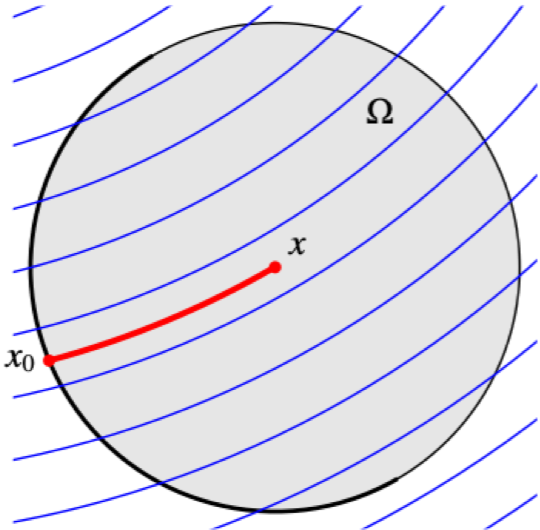
\includegraphics[width=0.4\columnwidth]{images/quasilinear}
\end{wrapfigure}

The PDE

\begin{align*}
    a(x,y,u)\frac{\partial u}{\partial x}+b(x,y,u)\frac{\partial u}{\partial y} = c(x,y,u)
\end{align*}

can be written in vector notation:

\begin{align*}
{\color{green}
\underbrace{
    \begin{pmatrix}
        a(x,y,u) \\
        b(x,y,u) \\
        c(x,y,u)
    \end{pmatrix}
}_{\vec t}
}
    \cdot
    {\color{black}
    \underbrace{
        \begin{pmatrix}
            \frac{\partial u}{\partial x} \\
            \frac{\partial u}{\partial y} \\
            -1
        \end{pmatrix}
    }_{\vec{n}}
    }
    &= 0
\end{align*}

where $\color{black}\vec{n}$ is a normal vector and $\color{green}\vec{t}$ is always tangential to the solution surface.
Therefore, we can elaborate a solution algorithm:
\begin{enumerate}
    \item{
        Using the Cauchy initial curve, we formulate
        \begin{align*}
            \vec{v}(s) = \begin{pmatrix}
                             v_x({\color{red}s} ) & v_y({\color{red}s}) & v_z({\color{red}s})
            \end{pmatrix}^T
        \end{align*}
        which is a point on the initial curve, parameterised by $s$.
    }
    \item{
        Find characteristic curves as solution of the ODEs

        \begin{align*}
            \frac{d}{d{\color{blue}t}}
            \begin{bmatrix}
                x({\color{blue}t}, {\color{red}s}) \\
                y({\color{blue}t}, {\color{red}s}) \\
                z({\color{blue}t}, {\color{red}s})
            \end{bmatrix}
            =
            \begin{bmatrix}
                a(x({\color{blue}t},{\color{red}s}), y({\color{blue}t},{\color{red}s}), z({\color{blue}t}, {\color{red}s})) \\
                b(x({\color{blue}t},{\color{red}s}), y({\color{blue}t},{\color{red}s}), z({\color{blue}t}, {\color{red}s})) \\
                c(x({\color{blue}t},{\color{red}s}), y({\color{blue}t},{\color{red}s}), z({\color{blue}t}, {\color{red}s}))
            \end{bmatrix}
        \end{align*}
        with
        \begin{align*}
            \begin{bmatrix}
                x({\color{blue}0}, {\color{red}s}) \\
                y({\color{blue}0}, {\color{red}s}) \\
                z({\color{blue}0}, {\color{red}s})
            \end{bmatrix}
            =
            \vec{v}({\color{red}s})
            =
            \begin{bmatrix}
                v_x({\color{red}s} ) \\
                v_y({\color{red}s})  \\
                v_z({\color{red}s})
            \end{bmatrix}
        \end{align*}
    }
    \item{
        Eliminate the variables {\color{blue}t} and {\color{red}s} and condense solution into a function $u(x, y)$:
        \begin{align*}
            \left.
            \begin{matrix}
                x=x({\color{blue}t},{\color{red}s}) \\
                y=y({\color{blue}t},{\color{red}s}) \\
                u=z({\color{blue}t},{\color{red}s})
            \end{matrix}
            \ \ \right\}
            \ u=u(x,y)
        \end{align*}
    }
\end{enumerate}
